\chapter{A convolutional neural network for CHIPS}
\label{chap:cvn}

\section{Deep neural network history and theory}

Neuron equation
\begin{equation}
    z^{(i)}=\boldsymbol{w}^{(i)}\cdot\boldsymbol{x}+b^{(i)}
\end{equation}

With activation function applied
\begin{equation}
    a_{i}(\boldsymbol{x})=\sigma_i(z^{(i)})
\end{equation}

\begin{figure}
    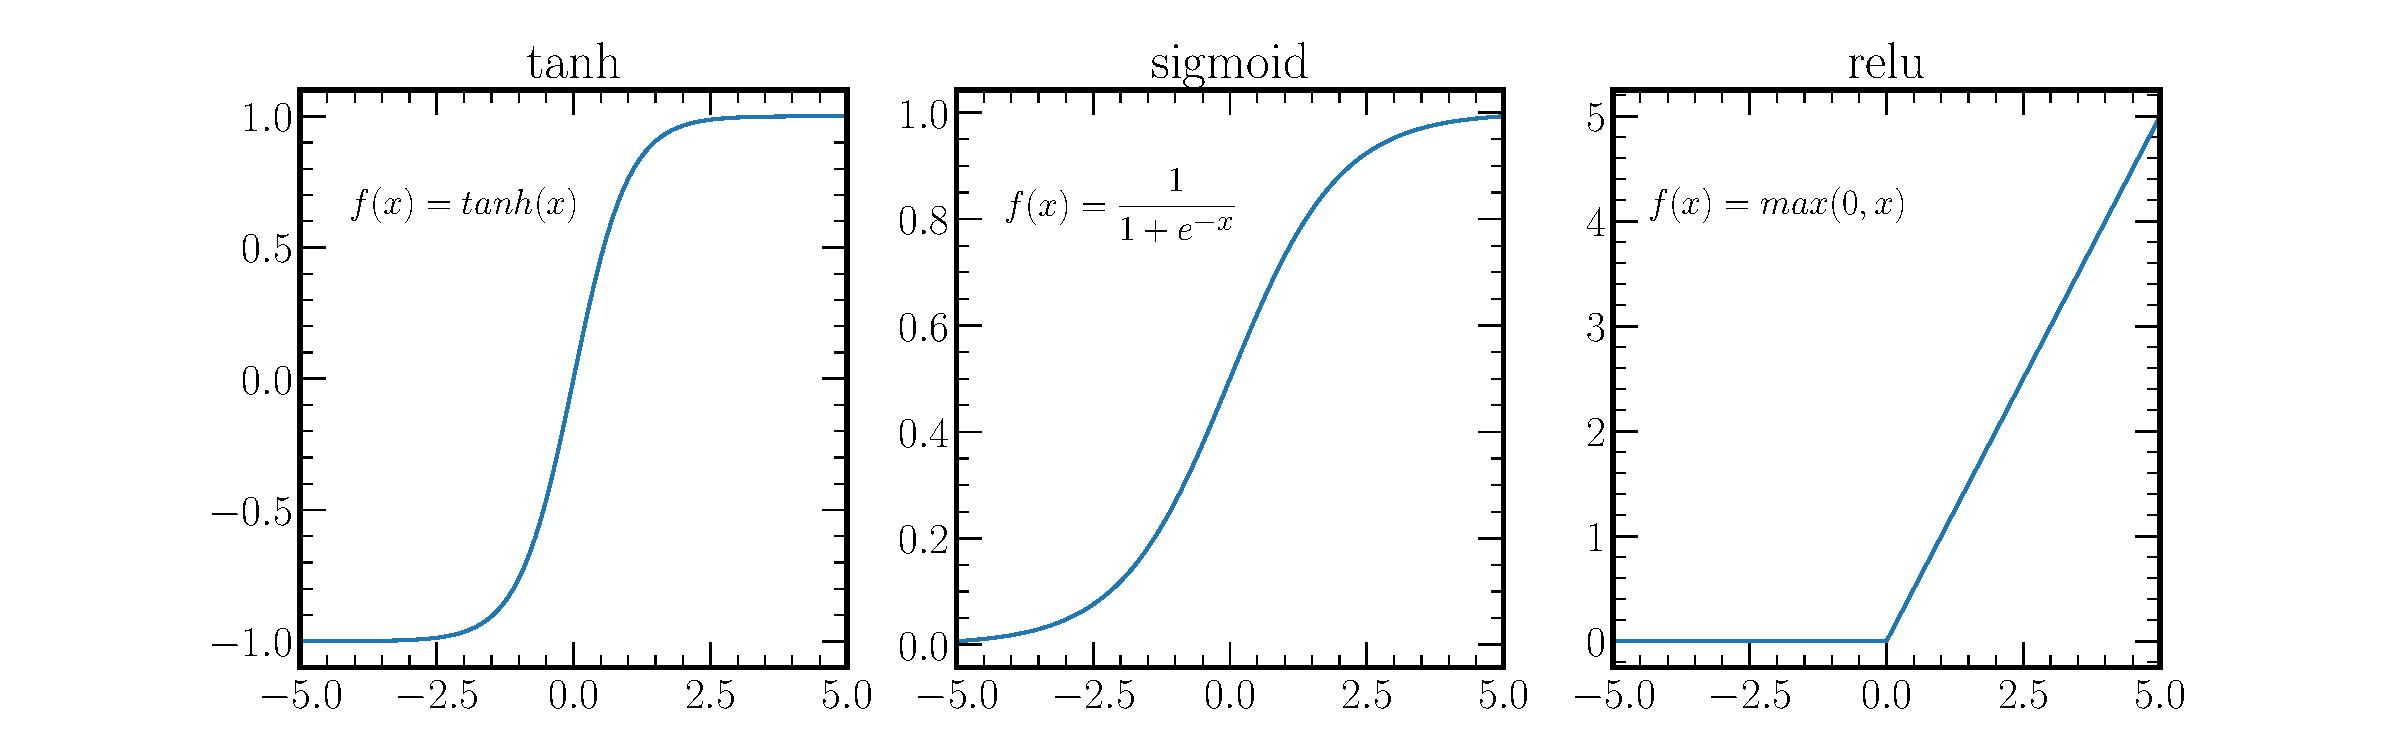
\includegraphics[width=\textwidth]{diagrams/6-cvn/activations.pdf}
    \caption[CKM Fitter constraints on \alphaCKM.]%
    {CKM Fitter constraints on \alphaCKM from combined \BToPiPi,
        \BToRhoPi and \BToRhoRho decay analyses.}
    \label{fig:activations}
\end{figure}

\begin{figure}
    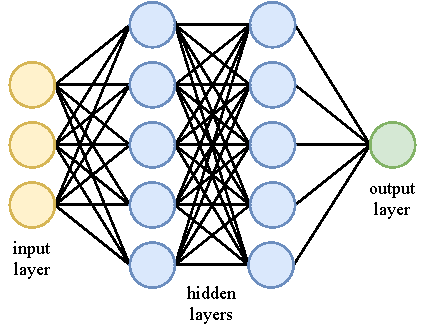
\includegraphics[width=\largefigwidth]{diagrams/6-cvn/network.pdf}
    \caption[CKM Fitter constraints on \alphaCKM.]%
    {Classic neural network architecture with neurons arrange in layers.
        The output of one layer acts as the input to the next layer until the output is reached.}
    \label{fig:network}
\end{figure}

\begin{figure}
    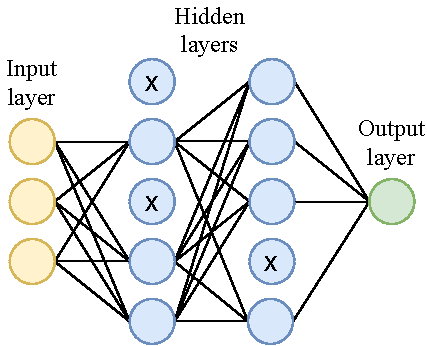
\includegraphics[width=\largefigwidth]{diagrams/6-cvn/dropout.pdf}
    \caption[CKM Fitter constraints on \alphaCKM.]%
    {CKM Fitter constraints on \alphaCKM from combined \BToPiPi,
        \BToRhoPi and \BToRhoRho decay analyses.}
    \label{fig:dropout}
\end{figure}


MSE
\begin{equation}
    E(\boldsymbol{w})=\frac{1}{n}\displaystyle\sum_{i=1}^{n}(y_{i}-\hat{y}_{i}(\boldsymbol{w}))^{2}
\end{equation}

Binary cross-entropy
\begin{equation}
    E(\boldsymbol{w})=-\displaystyle\sum_{i=1}^{n}y_{i}\log\hat{y}_{i}(\boldsymbol{w})+(1-y_{i})\log[1-\hat{y}_{i}(\boldsymbol{w})]
\end{equation}

categorical cross-entropy
\begin{equation}
    E(\boldsymbol{w})=-\displaystyle\sum_{i=1}^{n}\displaystyle\sum_{m=0}^{M-1}y_{im}\log\hat{y}_{im}(\boldsymbol{w})+(1-y_{im})\log[1-\hat{y}_{im}(\boldsymbol{w})]
\end{equation}

\begin{figure}
    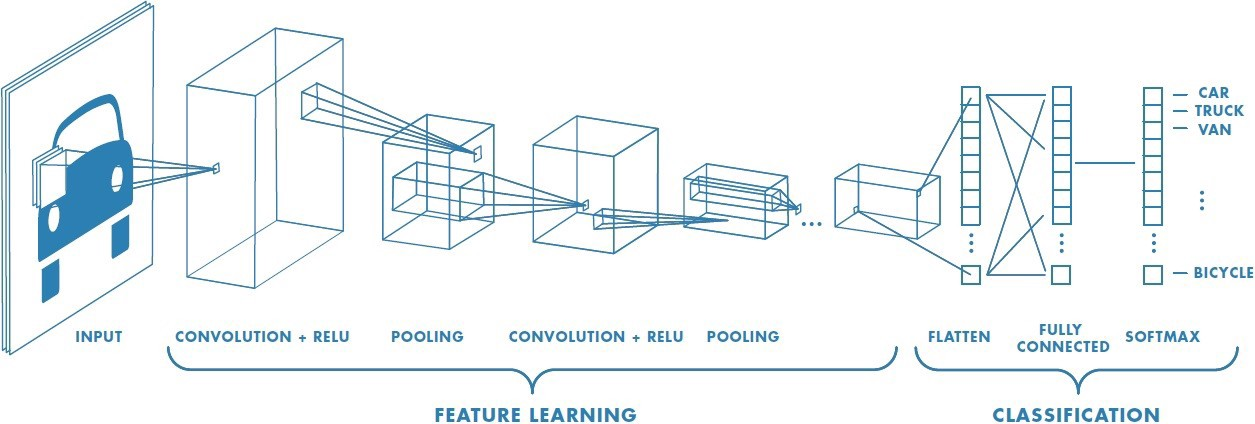
\includegraphics[width=\textwidth]{diagrams/6-cvn/conv_diagram.jpeg}
    \caption[CKM Fitter constraints on \alphaCKM.]%
    {CKM Fitter constraints on \alphaCKM from combined \BToPiPi,
        \BToRhoPi and \BToRhoRho decay analyses.}
    \label{fig:conv_diagram}
\end{figure}

\begin{figure}
    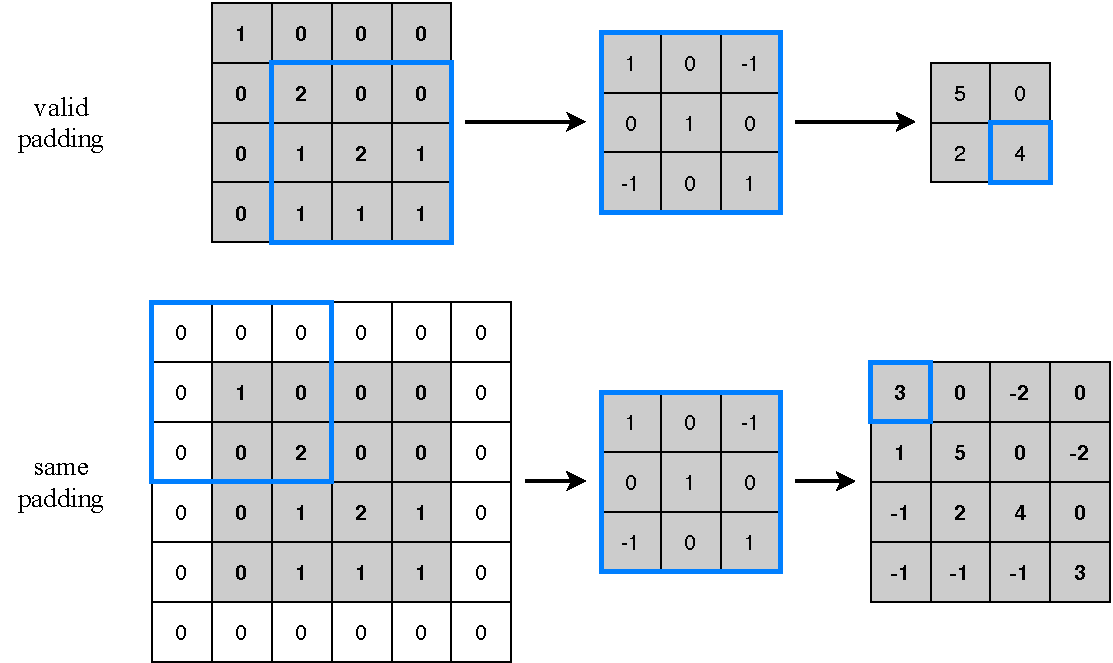
\includegraphics[width=\textwidth]{diagrams/6-cvn/conv_operation.pdf}
    \caption[CKM Fitter constraints on \alphaCKM.]%
    {CKM Fitter constraints on \alphaCKM from combined \BToPiPi,
        \BToRhoPi and \BToRhoRho decay analyses.}
    \label{fig:conv_operation}
\end{figure}

\begin{figure}
    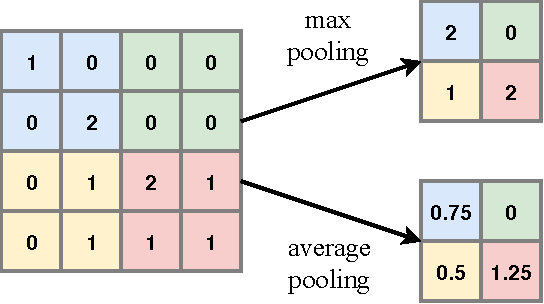
\includegraphics[width=\largefigwidth]{diagrams/6-cvn/pooling.pdf}
    \caption[CKM Fitter constraints on \alphaCKM.]%
    {CKM Fitter constraints on \alphaCKM from combined \BToPiPi,
        \BToRhoPi and \BToRhoRho decay analyses.}
    \label{fig:pooling}
\end{figure}



\section{Applications to HEP problems}

\begin{figure}
    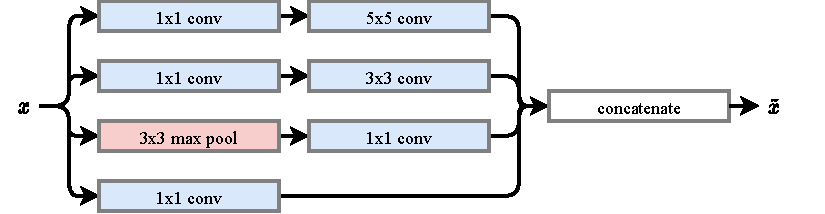
\includegraphics[width=\textwidth]{diagrams/6-cvn/inception.pdf}
    \caption[CKM Fitter constraints on \alphaCKM.]%
    {CKM Fitter constraints on \alphaCKM from combined \BToPiPi,
        \BToRhoPi and \BToRhoRho decay analyses.}
    \label{fig:inception}
\end{figure}

\begin{figure}
    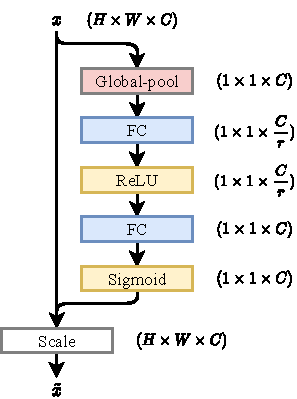
\includegraphics[width=\largefigwidth]{diagrams/6-cvn/se.pdf}
    \caption[CKM Fitter constraints on \alphaCKM.]%
    {CKM Fitter constraints on \alphaCKM from combined \BToPiPi,
        \BToRhoPi and \BToRhoRho decay analyses.}
    \label{fig:se}
\end{figure}

\begin{figure}
    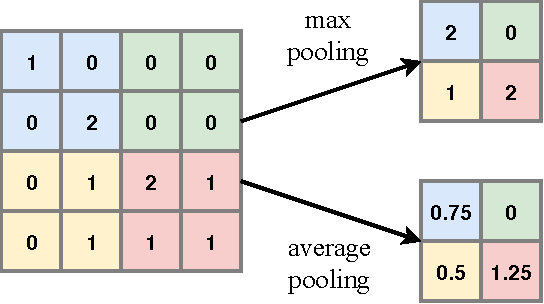
\includegraphics[width=\largefigwidth]{diagrams/6-cvn/pooling.pdf}
    \caption[CKM Fitter constraints on \alphaCKM.]%
    {CKM Fitter constraints on \alphaCKM from combined \BToPiPi,
        \BToRhoPi and \BToRhoRho decay analyses.}
    \label{fig:pooling}
\end{figure}

\begin{figure}
    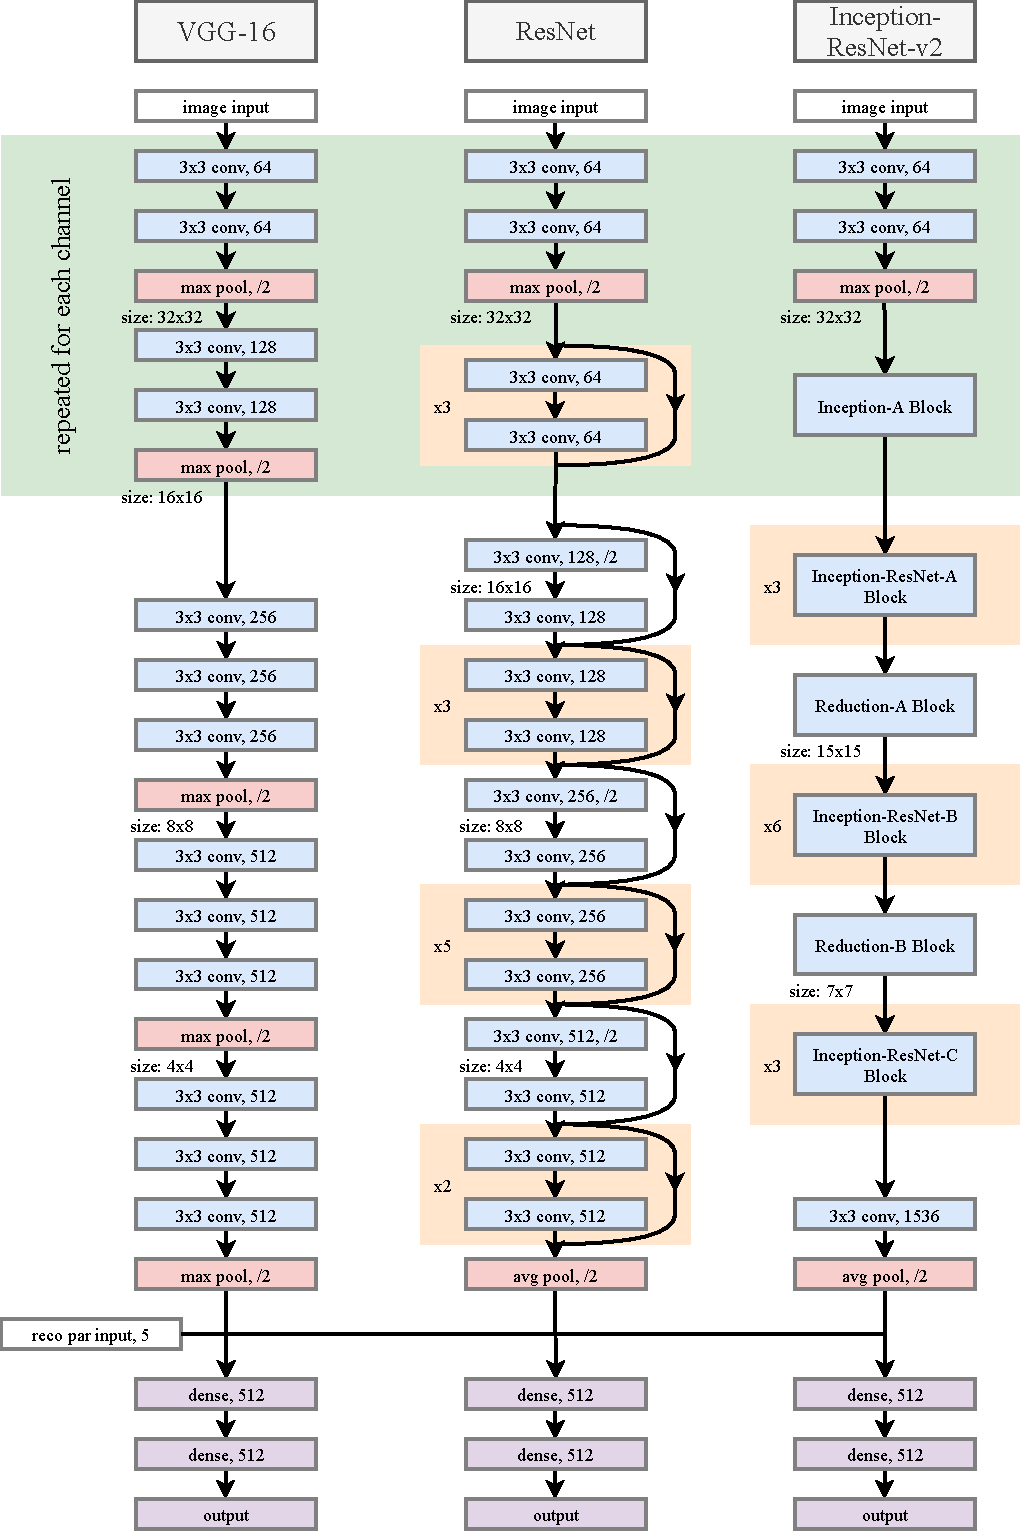
\includegraphics[width=\textwidth]{diagrams/6-cvn/chipsnet.pdf}
    \caption[CKM Fitter constraints on \alphaCKM.]%
    {CKM Fitter constraints on \alphaCKM from combined \BToPiPi,
        \BToRhoPi and \BToRhoRho decay analyses.}
    \label{fig:chipsnet}
\end{figure}



\section{Story of the chapter}

There are many standard ways that event classification and paramter (mainly energy) estimation are
usually done in HEP. These mainly include the reconstruction of objects and their associated parameters
wether these are clusters, tracks, jets or cherenkov rings. Typically these along with other constructed
features are then passed through a simple machine learning model for event or particle classification, or
combined in some other way for energy estimation.

While this has worked leveraging the enormous amount of work in machine learning especially deep learning
surely would prove valuable. The key thing that has been done is to move away from human engineered features
to machine learning models that discover the underlying features that work best in clasifiying of regressing
a particualar task.

Water chernkov detectors are especially paired to this task as the output from our detectors is essentially
an 'image' of the event and so classification models that work well on images shoud work well on
seperating our types of events.

Firstly, the principle issue with matching water cherenkov detectors and deep learning is representing the cylindrical
detector output of either a 2d flat map that a typically conv network can use as input of use a more complicated
graph network approach as some other people have tried. Typically people have just ignored the endcaps, but
this is not optimal as these contain nearing half the detected light in a standard CHIPS detector. Other appraoches
include the x+ x- approach. But as hited at by tomothy report, for a primarilly event classification task,
removing any distritions due to the detector shape is the most important things. Therefore, the approach of
veiwing the "image" from the interaction vertex point preserves the cherenkov ring strucutre as best possible.

The hough space is used to find this vertex and direction from which the images are produces, so it also made sense
to include this along with time as a seperate channel in the output. You can see fro the vertext position is best. Using
a more unformly distributes sample of events leads to a greater abiity to distinguish the types which is important
for subsequant energy reconstruction.

Many possible models have been developed for convolutional neural networks over th years.

Firstly, the principle issue with matching water cherenkov detectors and deep learning is representing the cylindrical
detector output of either a 2d flat map that a typically conv network can use as input of use a more complicated
graph network approach as some other people have tried. Typically people have just ignored the endcaps, but
this is not optimal as these contain nearing half the detected light in a standard CHIPS detector. Other appraoches
include the x+ x- approach. But as hited at by tomothy report, for a primarilly event classification task,
removing any distritions due to the detector shape is the most important things. Therefore, the approach of
veiwing the "image" from the interaction vertex point preserves the cherenkov ring strucutre as best possible.



\section{Intro, General theory and previous work}
- Standard water cherenkov analysis is via a likelihood hood fit to the ring assuming some event topology hypothesis.
This is used in super-k with fitqun and what has been previously implemented for CHIPS in the WCSimAnalysis package.

- Previous work in HEP has applied deep learning to a variety of problems...



- A MPL with a single hidden layer can be shown to apprximate any function arbitrarily accurately. Give REF for this.

- Conv is a set of 'filters' that when applied via scanning across an input image result in a feature map
- Pooling used as each layer requires less complexity and it is less important about the location and that the feature exists.


PLOT: Standard diagram of a convolutional neural network showing multiple filters etc...

REF:

\section{A CVN for \chips}

- Approaches in the past for event classification using CNNs for water cherenkov detectors have taken a few Approaches
to generating the input image representation.
- Projecting onto a 2d surface "outside" the detector
REF: Cern summer report in Ref.~\cite{theodore2016}




\section{Things to talk about}
- Convolutional neural network theory and history
- Recent uses in experiments
- CHIPS implementation tellig the story
- Explainability (ablation, clustering, layer weights etc...)

-


\section{Diagrams}

- Example event hit maps, showing the different possible channels for different types of event.
- True neutrino energy distributions for different categories for energy estimation.
- Network architecture plots.
- Neutrino energy and estimated neutrino energy distributions on same plots.
- reco-true/true neutrino energy distributions for the different event types, QEL, DIS, RES etc...
- Plot comparing lepton energy reconstruction between old reco and new estimation, just for nice CC events.
- Individual block diagrams for the different models I try + a squeeze-exitation diagram
- Arbitrary vs 8-bit precision for all the channels
- Example activation maps for a few events (explain)
- Number of events in each category within the training sample
- Training loss and accuracy vs epoch/iteration
- Classifier output plots
- Table of the final number of expected events and efficiency and purity of the signal at the chosen cut value (nuel and numu)
- t-SNE and PCA plots, nicely coloured
- Example events from the t-SNE plot, showing the different types
- Confusion matrices
- Parrallel coordinates plots for tuning the hyperparameters
- Time taken comparison with old reconstruction (just inference time for all stages)
- Final energy distribution of selected events given a number of years running

\section{References}

Cern summer report in Ref.~\cite{theodore2016}
CHIPS cosmic rate in Ref.~\cite{son2013}
Nova first CVN paper in Ref.~\cite{aurisano2016}
- CNN's have been widely applied in various computer vision tasks to solve image recongnition and analysis problems.
- The core problem in HEP is the correct categorisation of particle interactions
- This is usually done by reconstructing high-level componenets suh as clusters, tracks, showers, jets and rings. and
then summarising these objects energies, directions and shapes, these wuantities are then fed into k-nearest neighbours,
BDTs or MLPs to seperate sign from bkg.
- Prone to failure, mistakes in the reconstruction, and limitation to what has been implemented by humans.
- computer vision moved away from specifically constructed features to sing ML CNNs to discover the features.
- Manu HEP problems including water cherenkov detectors essentially result in an 'image' of an event, which are well suited to these tools.
- MLP are widely used in HEP,
Nova context enriched CVN paper in Ref.~\cite{psihas2019}
Nova energy recontruction CVN in Ref.~\cite{baldi2019}
Watchmal/Triumf Cherenkov variational autoencoders in Ref.~\cite{abhishek2019}
Daya bay paper in Ref.~\cite{racah2016}
SHiP GAN simulation paper in Ref.~\cite{ahdida2019}
New ideas with x+ x- mapping in Ref.~\cite{berns2020}
DUNE TDR in Ref.~\cite{abi2020}
Initial CNN visualisation paper in Ref.~\cite{zeiler2013}
Original t-SNE paper in Ref.~\cite{maaten2008}
Original 'dropout' paper in Ref.~\cite{hinton2012}
VGG paper in Ref.~\cite{simonyan2014}
Improved resnet paper in Ref.~\cite{he2016}
Inception-resnet paper in Ref.~\cite{szegedy2016}
Squeeze-and-excitation networks paper in Ref.~\cite{hu2017}
MobileNetV2 paper in Ref.~\cite{sandler2018}
Multi-task learning how to weight paper in Ref.~\cite{kendall2017}
Grad-CAM paper in Ref.~\cite{elvaraju2019}
Amazing machine learning for physicists thing in Ref.~\cite{mehta2019}
- Deep neural networks have emerged as one of the most powerful supervised learning techniques.
- They truly caught the attention of the wider ML communityr in 2012 when A. Krizhevsky, I, Sutskever and G. Hinton used a GPU to train
AlexNet, lowering the error rate on the image classification task ImageNet by 12%. 
- Such was the rapid pace of advance afterwards that the ResNet model acheived a 3.57\percent error just three years later.
- Many high level libraries have now been formed, predominently led by Tensorflow (from google) and pyTorch (from facebook) making it easier to quickly code and implemenetd DNNs.
- Neural networks are neural-inspired nonlinear models for supervised learning. Constructed from the basic building blocks of a "neuron".
-


\section{Reference notes}